\documentclass[t]{beamer}
%%\usetheme{Szeged}
\usetheme{Antibes}
\usecolortheme{dolphin}
\usepackage{cmap}					%поиск в pdf
\usepackage[T2A]{fontenc}			% кодировка
\usepackage[utf8]{inputenc}			% кодировка исходного текста
\usepackage[english,russian]{babel}	% локализация и переносы
%%% Работа с картинками
\usepackage{graphicx}  % Для вставки рисунков
\graphicspath{{images/}{images2/}}  % папки с картинками
\setlength\fboxsep{3pt} % Отступ рамки \fbox{} от рисунка
\setlength\fboxrule{1pt} % Толщина линий рамки \fbox{}
\usepackage{wrapfig} % Обтекание рисунков текстом

%%% Работа с таблицами
\usepackage{array,tabularx,tabulary,booktabs} % Дополнительная работа с таблицами
\usepackage{longtable}  % Длинные таблицы
\usepackage{multirow} % Слияние строк в таблице

%%% Программирование
\usepackage{etoolbox} % логические операторы

%%% Другие пакеты
\usepackage{lastpage} % Узнать, сколько всего страниц в документе.
\usepackage{soul} % Модификаторы начертания
\usepackage{csquotes} % Еще инструменты для ссылок
%\usepackage[style=authoryear,maxcitenames=2,backend=biber,sorting=nty]{biblatex}
\usepackage{multicol} % Несколько колонок

%%% Картинки
\usepackage{tikz} % Работа с графикой
\usepackage{pgfplots}
\usepackage{pgfplotstable}
\usepackage{hyperref}

\title{Senty}
\author{Балакший Андрей \and Сухочев Александр 
	\and \newline Куратор:Юрий Курочкин}
\date{19 мая 2015}
\institute[Computer Science Center]

\begin{document}
	\frame[plain]{\titlepage}
	
	
	\section{О проекте}
	\begin{frame}
		\frametitle{\insertsection}
		\textbf{Сентиментальная разметка коротких текстов с использованием "чистой"\ разметки обучающего множества.}
	\end{frame}
	
	
	\section{Вдохновение}
	\begin{frame}
		\frametitle{\insertsection}
		\textbf{Прочитали статью исследователей из Стэнфордского университета о сентиментальной разметке твитов. Они производили "грязную"\ разметку твитов(разметка по смайликам) и обучались по ней. \newline \newline}
        \hyperref[http://cs.stanford.edu/people/alecmgo/papers/TwitterDistantSupervision09.pdf]{\textbf{\underline{http://cs.stanford.edu/people/alecmgo/papers/} \newline \underline{TwitterDistantSupervision09.pdf}}} \pause
		\newline
        \newline
		\textbf{Захотелось чего-то аналогичного, но с русским языком и с "чистой"\ разметкой (разметкой вручную).}
	\end{frame}
	
	
	\section{Цель}
	\begin{frame}
		\frametitle{\insertsection}
		\textbf{Хотим по короткому тексту понимать настроение его автора.}
	\end{frame}
	
	
	\section{Этапы выполнения}
	\begin{frame}
    	
		\frametitle{\insertsection}
		\begin{itemize}
			\item \textbf{Найти источник материалов для обучения, содержащий высказывания людей на различные темы.}	
            \item \textbf{Разметить эти материалы вручную на положительные, отрицательные и нейтральные.}
			\item \textbf{Придумать различные признаки, которые помогут определять настроения авторов текстов (далее для упрощения будем называть эти признаки фичами).}
            \item \textbf{Реализовать машинное с учётом этих признаков.} 
		\end{itemize}
	\end{frame}
	
	
	\section{Получение материалов для обучения}
	\begin{frame}
		\frametitle{\insertsection}
		\textbf{Материалы для обучения спарсили с цитатника рунета bash.im. Для парсинга воспользовались питоновской библиотекой Beautiful Soup. \newline}
        
        ~~~~~~~~~~~~~~~~~~~~~~~ {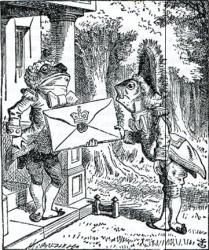
\includegraphics[scale = 0.6]{images/beautiful_soup.jpg}}
	\end{frame}
	
	
	\section{"Чистая" разметка обучающего множества}
	\begin{frame}
		\frametitle{\insertsection}
		\textbf{ Для удобства "чистой"\ разметки текстов (далее башей) написали приложение под Android, чтобы размечать баши где угодно и когда угодно.}
		
		~~~~~~~
		{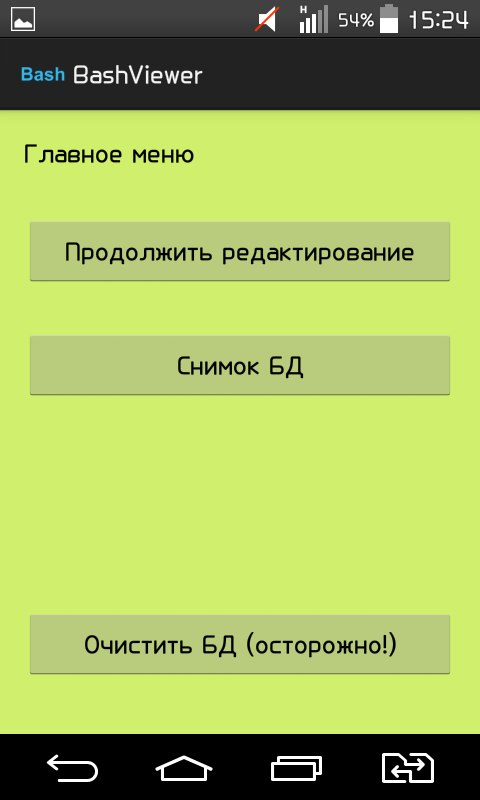
\includegraphics[scale = 0.17]{images/Bash1.jpg}
		
\includegraphics[scale = 0.17]{images/Bash2.jpg}
		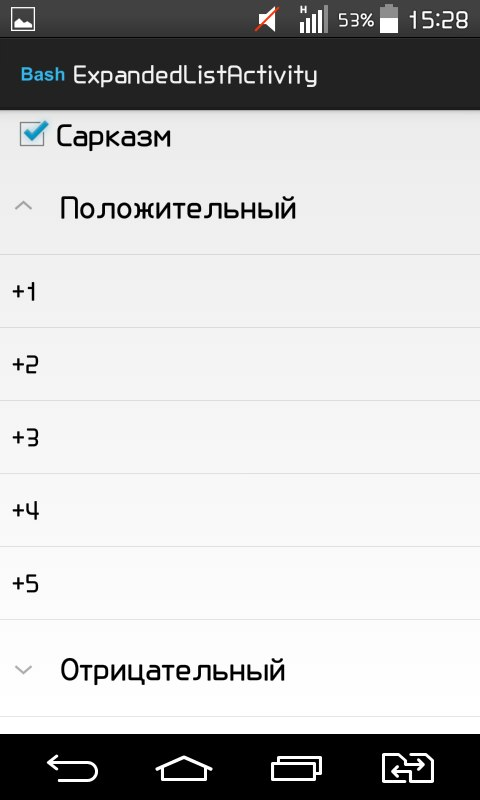
\includegraphics[scale = 0.17]{images/Bash3.jpg}}
	\end{frame}


	\section{Фичи}
    \begin{frame}
    	\frametitle{\insertsection}
        \textbf{Было создано множество фич, являющихся надстройками над стандартным экстрактором термов. В стандартном экстракторе мы просто убирали знаки препинания и нормализовывали слова с помощью питоновской библиотеки pymystem3.}
    \end{frame}

\section{Примеры работы некоторых фич}
	\begin{frame}
		\frametitle{\insertsection}
		\begin{itemize}
			\only<1-7>{\item \textbf{Исходный текст:} \newline "УЖАААСНО не люблю вставать по понедельникам и идти на работу ((((,... и по вторникам тоже ))"}
			
			\only<2-4>{\item \textbf{Работа стандартного экстрактора с pymystem3:} \newline"ужааасно не любить вставать по понедельник и идти на работа (((( и по вторник тоже ))"}
			
			\only<3-4>{\item \textbf{Добавление фичи, убирающей предлоги, союзы и местоимения:} \newline "ужааасно не любить вставать понедельник идти работа (((( вторник тоже ))"}
			
			\only<4>{\item \textbf{Добавление фичи, убирающей повторные буквы:} \newline "ужасно не любить вставать понедельник идти работа (((( вторник тоже ))"}
			
			\only<5-7>{\item \textbf{Добавление фичи, склеивающей "не"\ со словом, которому эта частица принадлежит:} \newline "ужасно нелюбить вставать понедельник идти работа (((( вторник тоже"}
			
			\only<6-7>{\item \textbf{Добавление фичи, выделяющей смайлики:} \newline "ужасно нелюбить вставать понедельник идти работа \alert{плохосмайл} вторник тоже \alert{хоросмайл}"}
            \only<7>{\item \textbf{Также были созданы фичи, выделяющие n-граммы, убирающие иностранные слова и многие другие.}}
		\end{itemize}
		
	\end{frame}


	\section{Выбор классификаторов}
	\begin{frame}
		\frametitle{\insertsection}
		
		\begin{itemize}
			\item 
			\textbf{Naive Bayes}
			\item
			\textbf{SVM}
			\item
			\textbf{MaxEntropy}			
		\end{itemize}
		
	\textbf{Для их реализации использовали питоновскую библиотеку scikit-learn.}
		

	\end{frame}	
	
	
	
	
	\section{Структура проекта}
	\begin{frame}
		\frametitle{\insertsection}
		\textbf{Для использования различных комбинаций фич с различными классификаторами была использована следующая структура.}
		
		
		~
		
		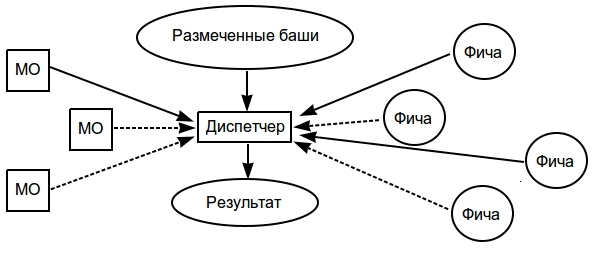
\includegraphics[scale=0.52]{images/TheManager.jpg}
	\end{frame}	
	
	
     \section{Результаты(Max Entropy)}
    \begin{frame}
		\frametitle{\insertsection}
    	\textbf{Фичи и точность:}
        \begin{itemize}
        	\item \textbf{Стандартный экстрактор без фич - 70,58\%}
            \item \textbf{+ убираем союзы - 70,85\%}
            \item \textbf{+ биграммы с "не"\ - 70,94\%}
        \end{itemize}
        \textbf{\newline \newline Итого удалось повысить точность на 0,36\%}
	\end{frame}
    
    
    
    \section{Результаты(SVM)}
    \begin{frame}
    	\frametitle{\insertsection}
%%%         \begin{array}{|l|r|} \hline {фичи} & {точность} \\ \hline {Стандартный\ %%%экстрактор} & {70,31\%} \\ \hline {+\ убираем\ повторяющиеся\ буквы} & {70,67\%} \\ %%%\hline {+\ убираем\ союзы} & {70,76\%}  \\ \hline {+\ биграммы\ с\ "не"} & {71,39\%} \\ 
%%%        \hline 
%%%        \end{array}
		\textbf{Фичи и точность:}
		\begin{itemize}
        	\item \textbf{Стандартный экстрактор без фич - 70,31\%}
            \item \textbf{+ убираем повторяющиеся буквы - 70,67\%}
            \item \textbf{+ убираем союзы - 70,76\%}
            \item \textbf{+ биграммы с "не"\ - 71,39\%}
        \end{itemize}
        \textbf{\newline \newline Итого удалось повысить точность на 1,08\%}
    \end{frame}
    
    \section{Результаты(Naive Bayes)}
   \begin{frame}
   		\frametitle{\insertsection}
        \textbf{Фичи и точность:}
        \begin{itemize}
        	\item \textbf{Стандартный экстрактор без фич - 65,83\%}
            \item \textbf{+ убираем повторяющиеся буквы - 66,37\%}
            \item \textbf{+ биграммы с "не"\ - 66,83\%}
            \item \textbf{+ убираем иностранные слова - 67,17\%}
            \item \textbf{+ выделяем смайлики - 67,26\%}
        \end{itemize}
        \textbf{\newline \newline Итого удалось повысить точность на 1,43\%}
   \end{frame}
    
    
    
	\section{Проблемы}
	
	\begin{frame}
		\frametitle{\insertsection}
		\begin{itemize}
			\item{\textbf{Малый объём выборки(примерно каждый четвёртый баш является эмоционально окрашенным, много сарказма, "чистая"\ разметка - дело не быстрое). Всего 9811 различных термов было выделено стандартным экстрактором.}}
			\item{\textbf{Сильный "перекос"\ в сторону отрицательных башей в обучающей выборке: из 1115 башей, имеющих эмоциональную окраску, 732 являются отрицательными (65.65\%).}}
		\end{itemize}
	\end{frame}

	\section{Дальнейшие перспективы}
	\begin{frame}
		\frametitle{\insertsection}
		\begin{itemize}
			\item
			\textbf{Двойная классификация: сначала классифицировать на нейтральное/с эмоциональной окраской, а потом уже эмоциональные на положительные/отрицательные. }
			\item
			\textbf{Прикрутить поиск по упоминаниям по базе башей для определения (с возможностью получения детальной информации с помощью какого-нибудь фильтра), сколько раз о предмете поиска отзывались положительно/отрицательно/нейтрально.}
			\item
			\textbf{Увеличение материала для обучения.} 
			
		\end{itemize}
		
	\end{frame}
		
	
	\section{Итоги практики}
	
	
	\begin{frame}
		\frametitle{\insertsection}
		\begin{itemize}
			\item \textbf{Работа в команде}
			\item \textbf{Изучение Python(Mystem, Scikit-learn, Beautiful Soup)}
			\item \textbf{Работа с GitHub}
			\item \textbf{Работа с \LaTeX (собственно создание самой презентации)}
		\end{itemize}
		~~~~~~~~~
		
\includegraphics[scale = 0.08]{images/git_hub.png}
		
\includegraphics[scale = 0.08]{images/latex-logo.png}
		
\includegraphics[scale = 0.2]{images/scikit_learn.png}
	\end{frame}
	
	
	
	
	\section{Спасибо за внимание}
	
	\begin{frame}
		\frametitle{\insertsection}
  		\hyperref[https://github.com/cscenter/senty]{\underline{https://github.com/cscenter/senty}}  
    
	
    \end{frame}
	
	
	
	
	
	
	
	
	
\end{document}\documentclass[t]{beamer}
%%\usetheme{Szeged}
\usetheme{Antibes}
\usecolortheme{dolphin}
\usepackage{cmap}					%поиск в pdf
\usepackage[T2A]{fontenc}			% кодировка
\usepackage[utf8]{inputenc}			% кодировка исходного текста
\usepackage[english,russian]{babel}	% локализация и переносы
%%% Работа с картинками
\usepackage{graphicx}  % Для вставки рисунков
\graphicspath{{images/}{images2/}}  % папки с картинками
\setlength\fboxsep{3pt} % Отступ рамки \fbox{} от рисунка
\setlength\fboxrule{1pt} % Толщина линий рамки \fbox{}
\usepackage{wrapfig} % Обтекание рисунков текстом

%%% Работа с таблицами
\usepackage{array,tabularx,tabulary,booktabs} % Дополнительная работа с таблицами
\usepackage{longtable}  % Длинные таблицы
\usepackage{multirow} % Слияние строк в таблице

%%% Программирование
\usepackage{etoolbox} % логические операторы

%%% Другие пакеты
\usepackage{lastpage} % Узнать, сколько всего страниц в документе.
\usepackage{soul} % Модификаторы начертания
\usepackage{csquotes} % Еще инструменты для ссылок
%\usepackage[style=authoryear,maxcitenames=2,backend=biber,sorting=nty]{biblatex}
\usepackage{multicol} % Несколько колонок

%%% Картинки
\usepackage{tikz} % Работа с графикой
\usepackage{pgfplots}
\usepackage{pgfplotstable}
\usepackage{hyperref}

\title{Senty}
\author{Балакший Андрей \and Сухочев Александр 
	\and \newline Куратор:Юрий Курочкин}
\date{19 мая 2015}
\institute[Computer Science Center]

\begin{document}
	\frame[plain]{\titlepage}
	
	
	\section{О проекте}
	\begin{frame}
		\frametitle{\insertsection}
		\textbf{Сентиментальная разметка коротких текстов с использованием "чистой"\ разметки обучающего множества.}
	\end{frame}
	
	
	\section{Вдохновение}
	\begin{frame}
		\frametitle{\insertsection}
		\textbf{Прочитали статью исследователей из Стэнфордского университета о сентиментальной разметке твитов. Они производили "грязную"\ разметку твитов(разметка по смайликам) и обучались по ней. \newline \newline}
        \hyperref[http://cs.stanford.edu/people/alecmgo/papers/TwitterDistantSupervision09.pdf]{\textbf{\underline{http://cs.stanford.edu/people/alecmgo/papers/} \newline \underline{TwitterDistantSupervision09.pdf}}} \pause
		\newline
        \newline
		\textbf{Захотелось чего-то аналогичного, но с русским языком и с "чистой"\ разметкой (разметкой вручную).}
	\end{frame}
	
	
	\section{Цель}
	\begin{frame}
		\frametitle{\insertsection}
		\textbf{Хотим по короткому тексту понимать настроение его автора.}
	\end{frame}
	
	
	\section{Этапы выполнения}
	\begin{frame}
    	
		\frametitle{\insertsection}
		\begin{itemize}
			\item \textbf{Найти источник материалов для обучения, содержащий высказывания людей на различные темы.}	
            \item \textbf{Разметить эти материалы вручную на положительные, отрицательные и нейтральные.}
			\item \textbf{Придумать различные признаки, которые помогут определять настроения авторов текстов (далее для упрощения будем называть эти признаки фичами).}
            \item \textbf{Реализовать машинное с учётом этих признаков.} 
		\end{itemize}
	\end{frame}
	
	
	\section{Получение материалов для обучения}
	\begin{frame}
		\frametitle{\insertsection}
		\textbf{Материалы для обучения спарсили с цитатника рунета bash.im. Для парсинга воспользовались питоновской библиотекой Beautiful Soup. \newline}
        
        ~~~~~~~~~~~~~~~~~~~~~~~ {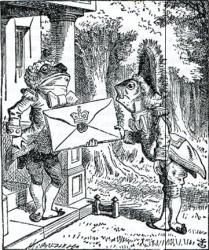
\includegraphics[scale = 0.6]{images/beautiful_soup.jpg}}
	\end{frame}
	
	
	\section{"Чистая" разметка обучающего множества}
	\begin{frame}
		\frametitle{\insertsection}
		\textbf{ Для удобства "чистой"\ разметки текстов (далее башей) написали приложение под Android, чтобы размечать баши где угодно и когда угодно.}
		
		~~~~~~~
		{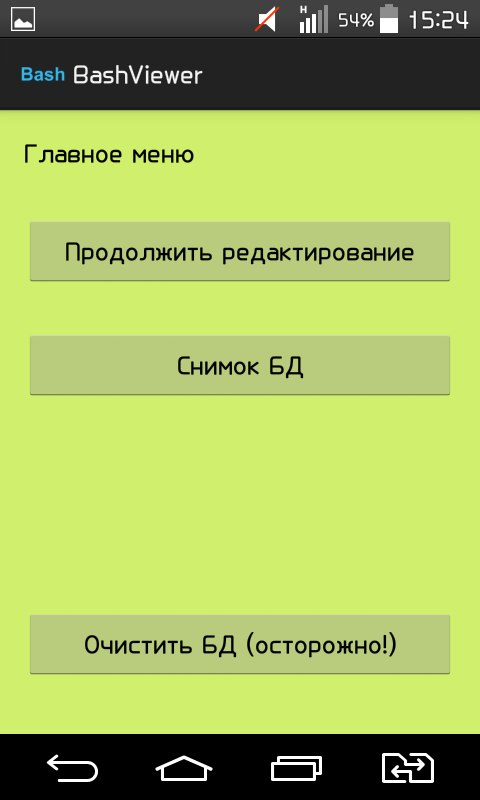
\includegraphics[scale = 0.17]{images/Bash1.jpg}
		
\includegraphics[scale = 0.17]{images/Bash2.jpg}
		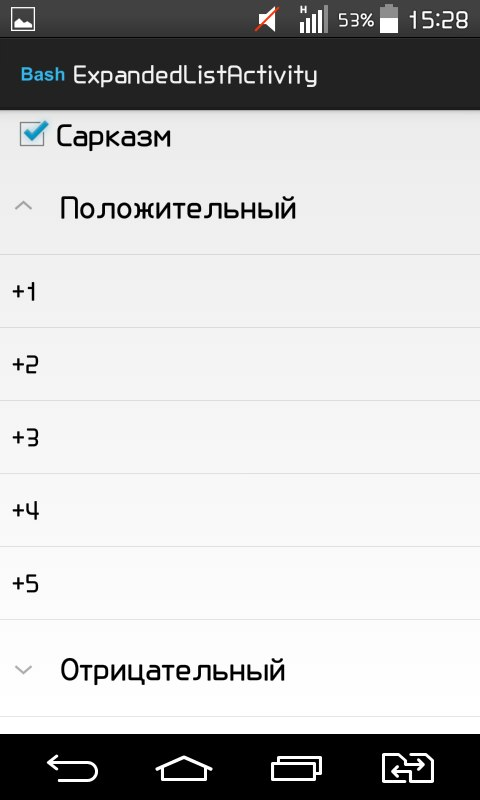
\includegraphics[scale = 0.17]{images/Bash3.jpg}}
	\end{frame}


	\section{Фичи}
    \begin{frame}
    	\frametitle{\insertsection}
        \textbf{Было создано множество фич, являющихся надстройками над стандартным экстрактором термов. В стандартном экстракторе мы просто убирали знаки препинания и нормализовывали слова с помощью питоновской библиотеки pymystem3.}
    \end{frame}

\section{Примеры работы некоторых фич}
	\begin{frame}
		\frametitle{\insertsection}
		\begin{itemize}
			\only<1-7>{\item \textbf{Исходный текст:} \newline "УЖАААСНО не люблю вставать по понедельникам и идти на работу ((((,... и по вторникам тоже ))"}
			
			\only<2-4>{\item \textbf{Работа стандартного экстрактора с pymystem3:} \newline"ужааасно не любить вставать по понедельник и идти на работа (((( и по вторник тоже ))"}
			
			\only<3-4>{\item \textbf{Добавление фичи, убирающей предлоги, союзы и местоимения:} \newline "ужааасно не любить вставать понедельник идти работа (((( вторник тоже ))"}
			
			\only<4>{\item \textbf{Добавление фичи, убирающей повторные буквы:} \newline "ужасно не любить вставать понедельник идти работа (((( вторник тоже ))"}
			
			\only<5-7>{\item \textbf{Добавление фичи, склеивающей "не"\ со словом, которому эта частица принадлежит:} \newline "ужасно нелюбить вставать понедельник идти работа (((( вторник тоже"}
			
			\only<6-7>{\item \textbf{Добавление фичи, выделяющей смайлики:} \newline "ужасно нелюбить вставать понедельник идти работа \alert{плохосмайл} вторник тоже \alert{хоросмайл}"}
            \only<7>{\item \textbf{Также были созданы фичи, выделяющие n-граммы, убирающие иностранные слова и многие другие.}}
		\end{itemize}
		
	\end{frame}


	\section{Выбор классификаторов}
	\begin{frame}
		\frametitle{\insertsection}
		
		\begin{itemize}
			\item 
			\textbf{Naive Bayes}
			\item
			\textbf{SVM}
			\item
			\textbf{MaxEntropy}			
		\end{itemize}
		
	\textbf{Для их реализации использовали питоновскую библиотеку scikit-learn.}
		

	\end{frame}	
	
	
	
	
	\section{Структура проекта}
	\begin{frame}
		\frametitle{\insertsection}
		\textbf{Для использования различных комбинаций фич с различными классификаторами была использована следующая структура.}
		
		
		~
		
		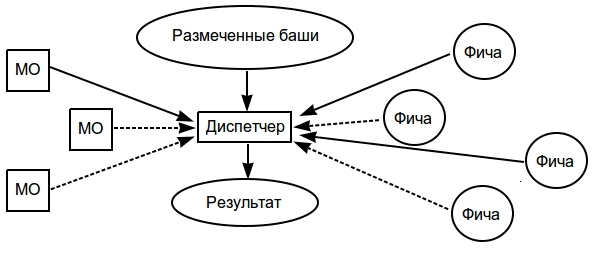
\includegraphics[scale=0.52]{images/TheManager.jpg}
	\end{frame}	
	
	
     \section{Результаты(Max Entropy)}
    \begin{frame}
		\frametitle{\insertsection}
    	\textbf{Фичи и точность:}
        \begin{itemize}
        	\item \textbf{Стандартный экстрактор без фич - 70,58\%}
            \item \textbf{+ убираем союзы - 70,85\%}
            \item \textbf{+ биграммы с "не"\ - 70,94\%}
        \end{itemize}
        \textbf{\newline \newline Итого удалось повысить точность на 0,36\%}
	\end{frame}
    
    
    
    \section{Результаты(SVM)}
    \begin{frame}
    	\frametitle{\insertsection}
%%%         \begin{array}{|l|r|} \hline {фичи} & {точность} \\ \hline {Стандартный\ %%%экстрактор} & {70,31\%} \\ \hline {+\ убираем\ повторяющиеся\ буквы} & {70,67\%} \\ %%%\hline {+\ убираем\ союзы} & {70,76\%}  \\ \hline {+\ биграммы\ с\ "не"} & {71,39\%} \\ 
%%%        \hline 
%%%        \end{array}
		\textbf{Фичи и точность:}
		\begin{itemize}
        	\item \textbf{Стандартный экстрактор без фич - 70,31\%}
            \item \textbf{+ убираем повторяющиеся буквы - 70,67\%}
            \item \textbf{+ убираем союзы - 70,76\%}
            \item \textbf{+ биграммы с "не"\ - 71,39\%}
        \end{itemize}
        \textbf{\newline \newline Итого удалось повысить точность на 1,08\%}
    \end{frame}
    
    \section{Результаты(Naive Bayes)}
   \begin{frame}
   		\frametitle{\insertsection}
        \textbf{Фичи и точность:}
        \begin{itemize}
        	\item \textbf{Стандартный экстрактор без фич - 65,83\%}
            \item \textbf{+ убираем повторяющиеся буквы - 66,37\%}
            \item \textbf{+ биграммы с "не"\ - 66,83\%}
            \item \textbf{+ убираем иностранные слова - 67,17\%}
            \item \textbf{+ выделяем смайлики - 67,26\%}
        \end{itemize}
        \textbf{\newline \newline Итого удалось повысить точность на 1,43\%}
   \end{frame}
    
    
    
	\section{Проблемы}
	
	\begin{frame}
		\frametitle{\insertsection}
		\begin{itemize}
			\item{\textbf{Малый объём выборки(примерно каждый четвёртый баш является эмоционально окрашенным, много сарказма, "чистая"\ разметка - дело не быстрое). Всего 9811 различных термов было выделено стандартным экстрактором.}}
			\item{\textbf{Сильный "перекос"\ в сторону отрицательных башей в обучающей выборке: из 1115 башей, имеющих эмоциональную окраску, 732 являются отрицательными (65.65\%).}}
		\end{itemize}
	\end{frame}

	\section{Дальнейшие перспективы}
	\begin{frame}
		\frametitle{\insertsection}
		\begin{itemize}
			\item
			\textbf{Двойная классификация: сначала классифицировать на нейтральное/с эмоциональной окраской, а потом уже эмоциональные на положительные/отрицательные. }
			\item
			\textbf{Прикрутить поиск по упоминаниям по базе башей для определения (с возможностью получения детальной информации с помощью какого-нибудь фильтра), сколько раз о предмете поиска отзывались положительно/отрицательно/нейтрально.}
			\item
			\textbf{Увеличение материала для обучения.} 
			
		\end{itemize}
		
	\end{frame}
		
	
	\section{Итоги практики}
	
	
	\begin{frame}
		\frametitle{\insertsection}
		\begin{itemize}
			\item \textbf{Работа в команде}
			\item \textbf{Изучение Python(Mystem, Scikit-learn, Beautiful Soup)}
			\item \textbf{Работа с GitHub}
			\item \textbf{Работа с \LaTeX (собственно создание самой презентации)}
		\end{itemize}
		~~~~~~~~~
		
\includegraphics[scale = 0.08]{images/git_hub.png}
		
\includegraphics[scale = 0.08]{images/latex-logo.png}
		
\includegraphics[scale = 0.2]{images/scikit_learn.png}
	\end{frame}
	
	
	
	
	\section{Спасибо за внимание}
	
	\begin{frame}
		\frametitle{\insertsection}
  		\hyperref[https://github.com/cscenter/senty]{\underline{https://github.com/cscenter/senty}}  
    
	
    \end{frame}
	
	
	
	
	
	
	
	
	
\end{document}